\chapter{Background}
\label{chap:background}
\section{Docker}
Docker \cite{Docker} is an open-source project container engine. It provides an additional layer of abstraction and automation of operating-system-level virtualization in Linux. Moreover, Docker has extra image management and layered file system to optimize the performance of container and reduce disk space. Docker images and Docker containers share the same image layer file if they have the same data. When Docker creates container, Docker will create a writable layer that allow the container application to change file system. Docker has two parts; Docker Client and Docker Daemon.

\begin{figure}[h]
\begin{center}
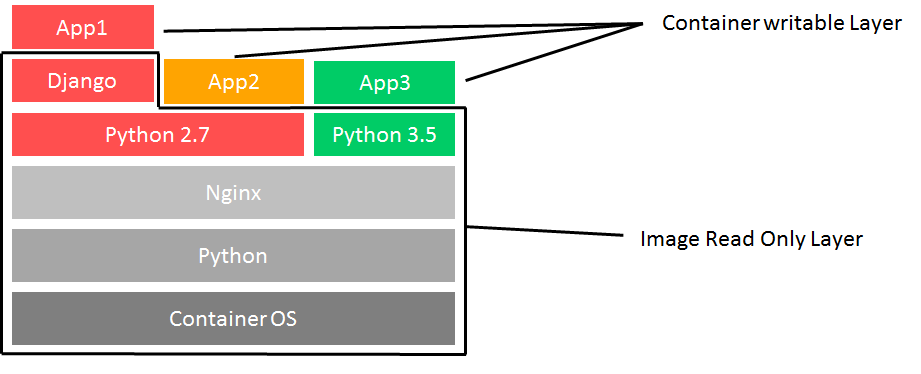
\includegraphics[width=15cm]{figure/layered_file_system.png}
\end{center}
\caption{Docker layered file system}
\label{fig:Docker layered file system}
\end{figure}

\begin{figure}[h]
\begin{center}
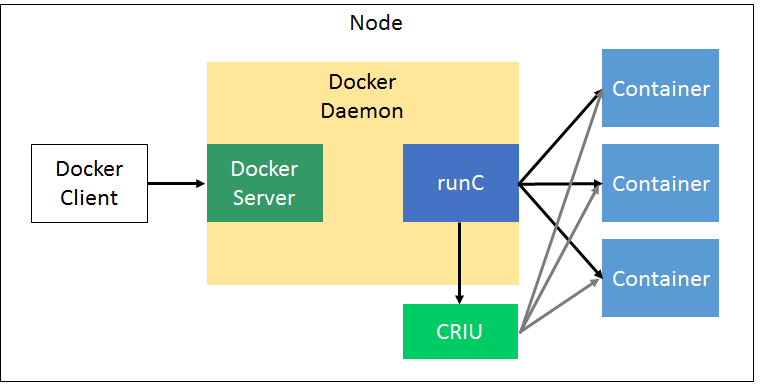
\includegraphics[width=10cm]{figure/single_node.png}
\end{center}
\caption{Single node Docker}
\end{figure}

\subsection{Docker Client}
Docker is typical client/server architecture application.
Docker Client is a \linebreak CLI (Client Line Interface) in Docker.
Docker uses Docker Client to send and receive requests to Docker Daemon. Also, Docker supports remote RESTful API to send and receive HTTP requests to Docker Daemon.
In additional, it has been implemented by more than 10 programming languages.

\subsection{Docker Daemon}
Docker Daemon is a daemon that runs as system service. It has three of the most importance features: 
\begin{itemize}
    \item Receive and handle requests from Docker Clients.
    \item Manage containers.
    \item Manage container images.
\end{itemize}
When Docker Daemon is running, it will run a server that receives requests from Docker Clients or remote RESTful API. After receiving requests, server will pass the requests by router to find the handler to handle the requests. By default, Docker Daemon listens to UNIX socket requests, it serves root permission, or docker group membership. Whenever user wants Docker Daemon to listen to remote RESTful API or Docker Swarm requests, it has to enable the TCP socket.

\subsection{runC}
When Docker came into being, Docker used LXC as its container execution environment. After Docker version 0.9, Docker dropped LXC but used libcontainer as its default execution environment.
runC is basically a repackaging of libcontainer, which is a CLI tool for running containers according to the OCI(Open Container Initiative) specification. It doesn't need any dependency from the operating system, it can control the Linux Kernel, including namespace, cgroups, apparmor, network, capabilities, firewall, etc.
runC provides a standard interface to support the containers management that Docker can use it to control the containers.

\begin{figure}[h]
\begin{center}
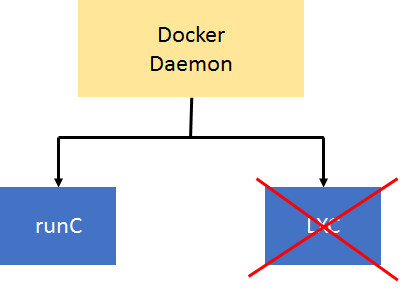
\includegraphics[width=6cm]{figure/docker_LXC.png}
\end{center}
\caption{Docker Daemon execution environment with runC and LXC}
\label{fig:docker_LXC}
\end{figure}

\section{CRIU}
CRIU \cite{CRIU} (Checkpoint/Restore in Userspace) stands for Checkpoint and Restore in User Space, creates a complete snapshot of the state of a process, including things like memory contents, file descriptors, and even open TCP connections. It can be used for suspending and resuming processes, or migrating them from one machine to another.

\subsection{Checkpoint}
\subsubsection{Pre-dump}
\subsubsection{Checkpoint}

\subsubsection{Restore}

\section{Docker Swarm}
Docker Swarm \cite{DockerSwarm} is a native clustering for Docker. It gathers several Docker engines together into one virtual Docker engine. Docker Swarm serves standard Docker API, so it can be connected by Dokku, Docker Machine, Docker Compose, Jenkins, DockerUI, Drone, etc. Of course, it also supports Docker Client as well.

In Docker Swarm, it has two components which are Swarm Manager and Swarm Node. Swarm Manager is the manager which handles Docker Client and RESTful API requests and manages multiple Docker Nodes' resources. Docker Node is an agent which sends heartbeat to Discovery Service to ensure Docker Daemon is alive in the cluster.

\begin{figure}[h]
\begin{center}
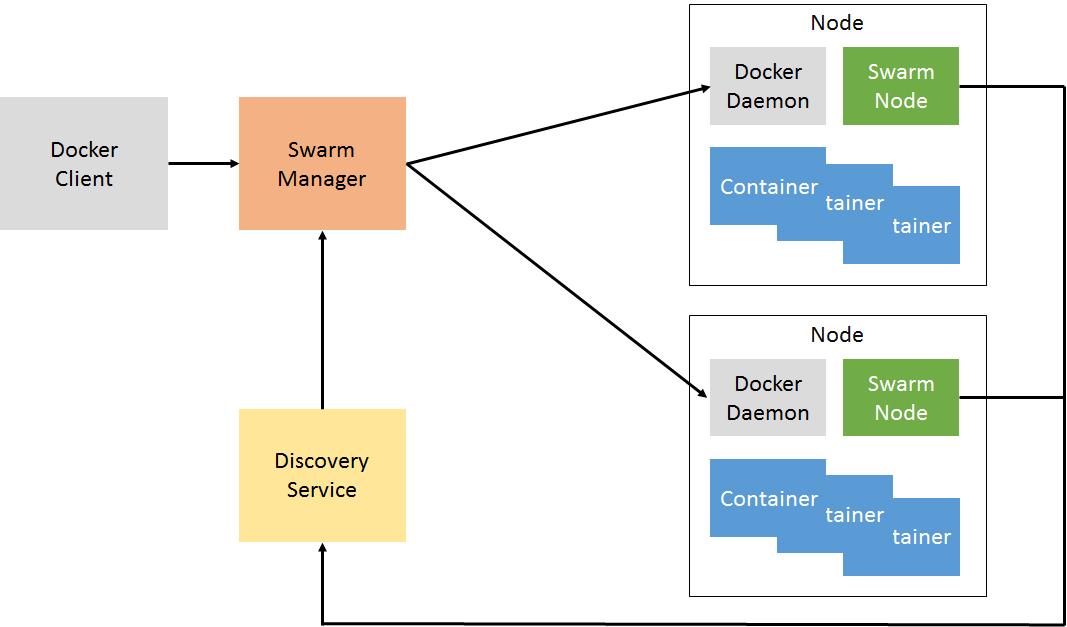
\includegraphics[width=15cm]{figure/swarm_docker.png}
\end{center}
\caption{Docker Swarm architecture}
\end{figure}

\subsection{Discovery services}
Docker Swarm provides multiple Discovery Services backends. They are used to discover the nodes in the cluster. There are:
\begin{itemize}
    \item Using a distributed key/value store, like Consul, Etcd and Zookeeper.
    \item A static file or list of nodes.
    \item Docker Hub as a hosted discovery service.
\end{itemize}
Otherwise, it also supports any modules that satisfy Discovery API interface.

\subsection{Scheduler}
Docker Swarm scheduler decides which nodes to use when creating and running a container. It has two steps:
First, the scheduler follows user's filters to decide which nodes conform to it.
Secondly, it undergoes multiple strategies to select the best node in the cluster.

\subsubsection{Filter}
Filters are divided into two categories;
Container configuration filters operate on characteristics of containers, or on the availability of images on a host.
Node filters operate on characteristics of the Docker host or on the configuration of the Docker Daemon.

The container configuration filters are:
\begin{itemize}
    \item Affinity
    \item Dependency
    \item Port filter
\end{itemize}
The node filters are:
\begin{itemize}
    \item Constraint
    \item Container slots
    \item Health filter
\end{itemize}

\subsubsection{Strategies}
The Docker Swarm scheduler features multiple strategies for ranking nodes. Docker Swarm currently supports these values:
\begin{itemize}
    \item Spread
    \item Binpack
    \item Random
\end{itemize}
Spread and Binpack strategies compute rank according to a node’s available CPU, its RAM, and the number of containers it has. It selects a node at random.
Under the Spread strategy, Swarm chooses the node with the least number of containers.
The Binpack strategy chooses the node which has executed most containers.
The Random strategy uses no computation and chooses nodes at random regardless of their available CPU or RAM.

\subsection{High availability of Swarm Manager}
In Docker Swarm, Swarm Manager responds to the cluster and manages the resources of multiple Docker Nodes at scale. If Swarm Manager dies, we have to create a new one and deal with the interruption of service.

The High availability feature allows Docker Swarm has multiple Swarm Manager instances. We can create a primary manager and multiple replica instances.
Whenever we send requests to replica instances, it will be automatically proxied to the primary manager.
In addition, if the primary manager fails, the other replica instances will lead a new primary manager.

\subsection{High availability of Docker Swarm containers}
In Docker Swarm, it has a rescheduling policy. As we set the reschedule policy when we start a container, whenever Swarm nodes fail, Swarm Manager will restart all of the containers to another alive Swarm Nodes.
